\section{Exercice 3 : Transformation d'une image}
\begin{enumerate}
  \item
        \q{Réaliser et faire afficher une symétrie par rapport à l'axe horizontal.}\\
        Je définis la symétrie verticale :
        \codeFromFile{section-03/q1-1.py}
        Et j'affiche le tout :
        \codeFromFile{section-03/q1-2.py}
        \begin{center}
          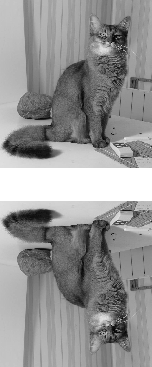
\includegraphics[scale=0.5]{section-03/q1-3.png}
        \end{center}

  \item
        \q{Réaliser et faire afficher une symétrie par rapport à l'axe vertical.}\\
        Pareil :
        \codeFromFile{section-03/q2-1.py}
        \codeFromFile{section-03/q2-2.py}
        \begin{center}
          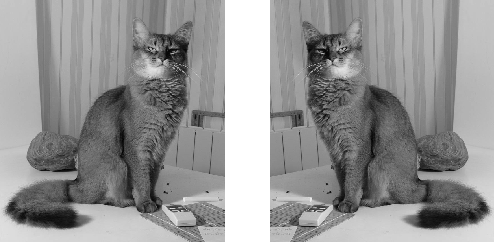
\includegraphics[scale=0.4]{section-03/q2-3.png}
        \end{center}

  \item
        \q{Réaliser et faire afficher une rotation de 20\%.}\\
        Je définis : \il{def cos(x): return np.cos(x)} et
        \il{def sin(x): return np.sin(x)} pour un peu plus de clareté.
        Puis je définis \il{rotation} :
        \codeFromFile{section-03/q3-1.py}
        \begin{center}
          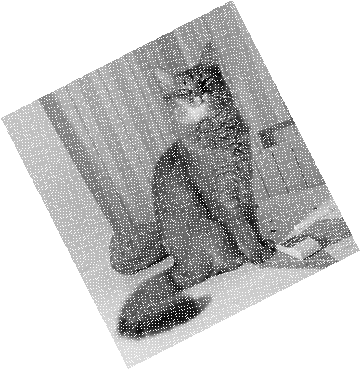
\includegraphics[scale=0.4]{section-03/q3-2.png}
        \end{center}

  \item
        \q{Faire afficher l'image en négatif.}
        \codeFromFile{section-03/q4-1.py}
        \begin{center}
          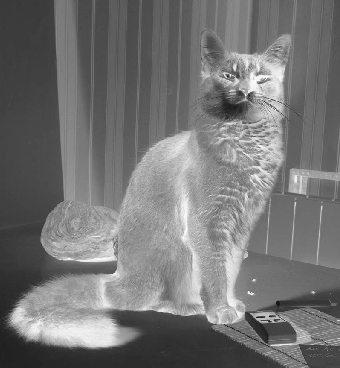
\includegraphics[scale=0.4]{section-03/q4-2.png}
        \end{center}

  \item
        \q{Faire afficher l'image en négatif.}
        \codeFromFile{section-03/q5-1.py}
        \begin{center}
          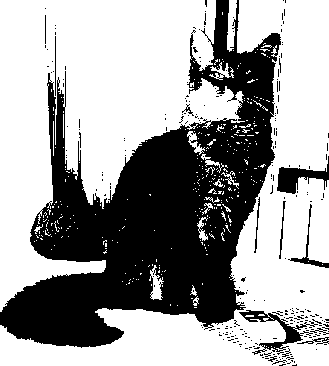
\includegraphics[scale=0.4]{section-03/q5-2.png}
        \end{center}

\end{enumerate}
